\documentclass[11pt]{article}
\usepackage[utf8]{inputenc}\usepackage[T1]{fontenc}
\usepackage{amsmath,amssymb,amsthm}\usepackage[margin=1in]{geometry}
\usepackage{graphicx}\usepackage{booktabs}
\usepackage[hidelinks]{hyperref}
\newtheorem{theorem}{Theorem}
\newtheorem{prediction}{Prediction}

\title{The Tuple-Size Law at $m=5$:\\
Resolving the Sparse Regime}
\author{Ruqing Chen\\
\small GUT Geoservice Inc., Montreal, Quebec, Canada\\
\small \texttt{ruqing@hotmail.com}}
\date{\today}

\begin{document}
\maketitle

\begin{abstract}
Part~XVIII confirmed the tuple-size law $d\ln\rho_m/d\ell\to-m$ at $m=4$ and
predicted the prime quintuplet ($m=5$): slope $-5$, ratio $5{:}2$ against the
twin. We test it, and in doing so meet the regime the law had been heading
toward. At the baseline $S_9\!\to\!S_{10}$ the quintuplet---only $2{,}936$
members on $S_9$---reads slope $-5.43$ and ratio $2.62$, overshooting the
$2.5\pm0.06$ bound: the prediction's own caveat, that sparsity would pull the
estimate up, made flesh. Descending one shell to $S_{10}\!\to\!S_{11}$, where the
quintuplet count recomputed from sieve primitives is $102{,}254$ (with the twin
counted in the same pass, $196{,}963{,}369$), the slope falls to $-5.065\pm0.09$
and the ratio to $2.4488\pm0.042$---inside the bound, on the law. The physics
obeyed the mathematics: the theory said depth would correct the sparse estimate,
and it did, to $-5.065$. The ladder is now ironclad at four rungs,
$m=2,3,4,5$, with $|d\ln\rho_m/d\ell|=\kappa\,m$ and ratios
$1:1.5011:2.0145:2.4488$ against $1:\tfrac32:2:\tfrac52$. The count-aware
estimator introduced in Part~XVIII passed its stress test in the sparsest regime
yet reached. As ever: Hardy--Littlewood inputs, first moments only, the
$\omega$-variance left open, no infinitude claimed. This closes the empirical
mining of the series. We leave $m=6$---slope $-6$, ratio $3{:}1$, requiring
shells beyond $S_{11}$---as the open challenge for supercomputer centres.
\end{abstract}

\section{The ladder and its last rung}

Across Parts~XVII and XVIII the tuple-size law accumulated three points: in the
proper depth $\ell=\ln\ln X$ a prime $m$-tuple obeys $d\ln\rho_m/d\ell\to-m$, with
$m=2,3,4$ collinear through the origin, $|d\ln\rho_m/d\ell|=\kappa\,m$, ratios
$1:\tfrac32:2$~\cite{ChenXVII,ChenXVIII}. Part~XVIII made $m=5$ a prediction and
flagged precisely the difficulty it would bring: the quintuplet is roughly an
order of magnitude rarer than the quadruplet, so the test ``will lean entirely on
the count-aware estimator and may require shells beyond $S_{10}$.'' This paper is
that test, and it is the rung where the sparse regime---which the law had been
approaching with each $m$---finally has to be confronted head-on.

\section{The quintuplet on the skeleton}

The densest admissible $5$-tuple is $(p,p+2,p+6,p+8,p+12)$. On the $6N$ skeleton,
with $p=6N-1$,
\[
  (6N-1,\,6N+1,\,6N+5,\,6N+7,\,6N+11),
\]
the two complete twin centres $N,N+1$ of the quadruplet together with the left
wing of $N+2$, with singular series $\mathfrak{S}(0,2,6,8,12)$. As before we test
only the exponent; the Hardy--Littlewood heuristic~\cite{HL} gives
$\rho_5(X)\approx A_5/(\ln X)^5$, the constant $A_5$ fixing only the intercept.

\section{Sparsity bites: the $S_9\!\to\!S_{10}$ reading}

Counts at $S_2$--$S_8$ are recomputed from a segmented value sieve; the production
shells $S_9,S_{10},S_{11}$ are recomputed independently. On $S_9$ the quintuplet
has just $2{,}936$ centres and on $S_{10}$ only $16{,}570$, so the local
log-density carries $\sim2\%$ and $\sim0.8\%$ Poisson noise and the
$S_9\!\to\!S_{10}$ slope inherits a standard error of $\pm0.19$:
\[
  \left.\frac{d\ln\rho_5}{d\ell}\right|_{S_9\to S_{10}}=-5.43,
  \qquad \text{ratio to twin } 2.62\pm0.09 .
\]
This overshoots the integer $-5$ and the bound $2.5\pm0.06$. The count-aware
(Poisson-weighted) intercept is $-5.36$. The cause is not a failure of the law
but exactly the effect Part~XVIII anticipated: at $m=5$ the logarithmic tail is
large and the sparsity noise compounds it, both pulling the finite-scale estimate
\emph{up} (steeper than $-5$). The remedy the prediction named was depth.

\section{Depth resolves it: the $S_{10}\!\to\!S_{11}$ reading}

We descended one shell. Counting the quintuplet \emph{and} the twin in a single
segmented-sieve pass at $S_{11}$ gives
\[
  \#\{\text{quintuplet}\}=102{,}254,\qquad
  \#\{\text{twin}\}=196{,}963{,}369,
\]
the twin reproducing the Part~I tables exactly. With
$\Delta\ell_{S_{10}\to S_{11}}=\ln(11/10)=0.09531$ the deeper, better-sampled
slope is
\[
  \boxed{\ \left.\frac{d\ln\rho_5}{d\ell}\right|_{S_{10}\to S_{11}}
  = -5.065\pm0.09,\qquad \text{ratio to twin } 2.4488\pm0.042\ }
\]
inside the $2.5\pm0.06$ bound, with the twin slope $-2.068$ from the same pass.
The tail has shrunk from $+0.43$ to $+0.065$---deeper means smaller tail, just as
in the $m=2,3,4$ cases---and the ratio noise from $\pm0.09$ to $\pm0.04$. The
prediction was specific (sparsity pulls the $S_{10}$ estimate up; depth corrects
it) and the data obeyed it: $-5.43\to-5.065$, $2.62\to2.449$. Where Part~XVIII's
quadruplet needed only a sharper estimator, the quintuplet needed the estimator
\emph{and} the extra shell---the first rung at which both tools of the sparse
regime were necessary, and both worked.

\begin{table}[h]\centering\small
\begin{tabular}{lccc}
\toprule
pattern & $m$ & $|d\ln\rho_m/d\ell|$ (deepest reliable) & ratio to twin (target)\\
\midrule
twin       & 2 & $2.072$ \ ($S_9\!\to\!S_{10}$)            & $1.0000$\\
triplet    & 3 & $3.111$ \ ($S_9\!\to\!S_{10}$)            & $1.5011$ \ ($\tfrac32$)\\
quadruplet & 4 & $4.175$ \ ($S_9\!\to\!S_{10}$)            & $2.0145$ \ ($2$)\\
quintuplet & 5 & $5.065$ \ ($S_{10}\!\to\!S_{11}$)         & $2.4488$ \ ($\tfrac52$)\\
\bottomrule
\end{tabular}
\caption{The four-rung ladder. The quintuplet is quoted at $S_{10}\!\to\!S_{11}$
(its $S_9\!\to\!S_{10}$ value $-5.43$ is sparsity-limited); the others at
$S_9\!\to\!S_{10}$. Ratios $1:1.5011:2.0145:2.4488$ against $1:\tfrac32:2:\tfrac52$.}
\label{tab:ladder}
\end{table}

\begin{figure}[h]\centering
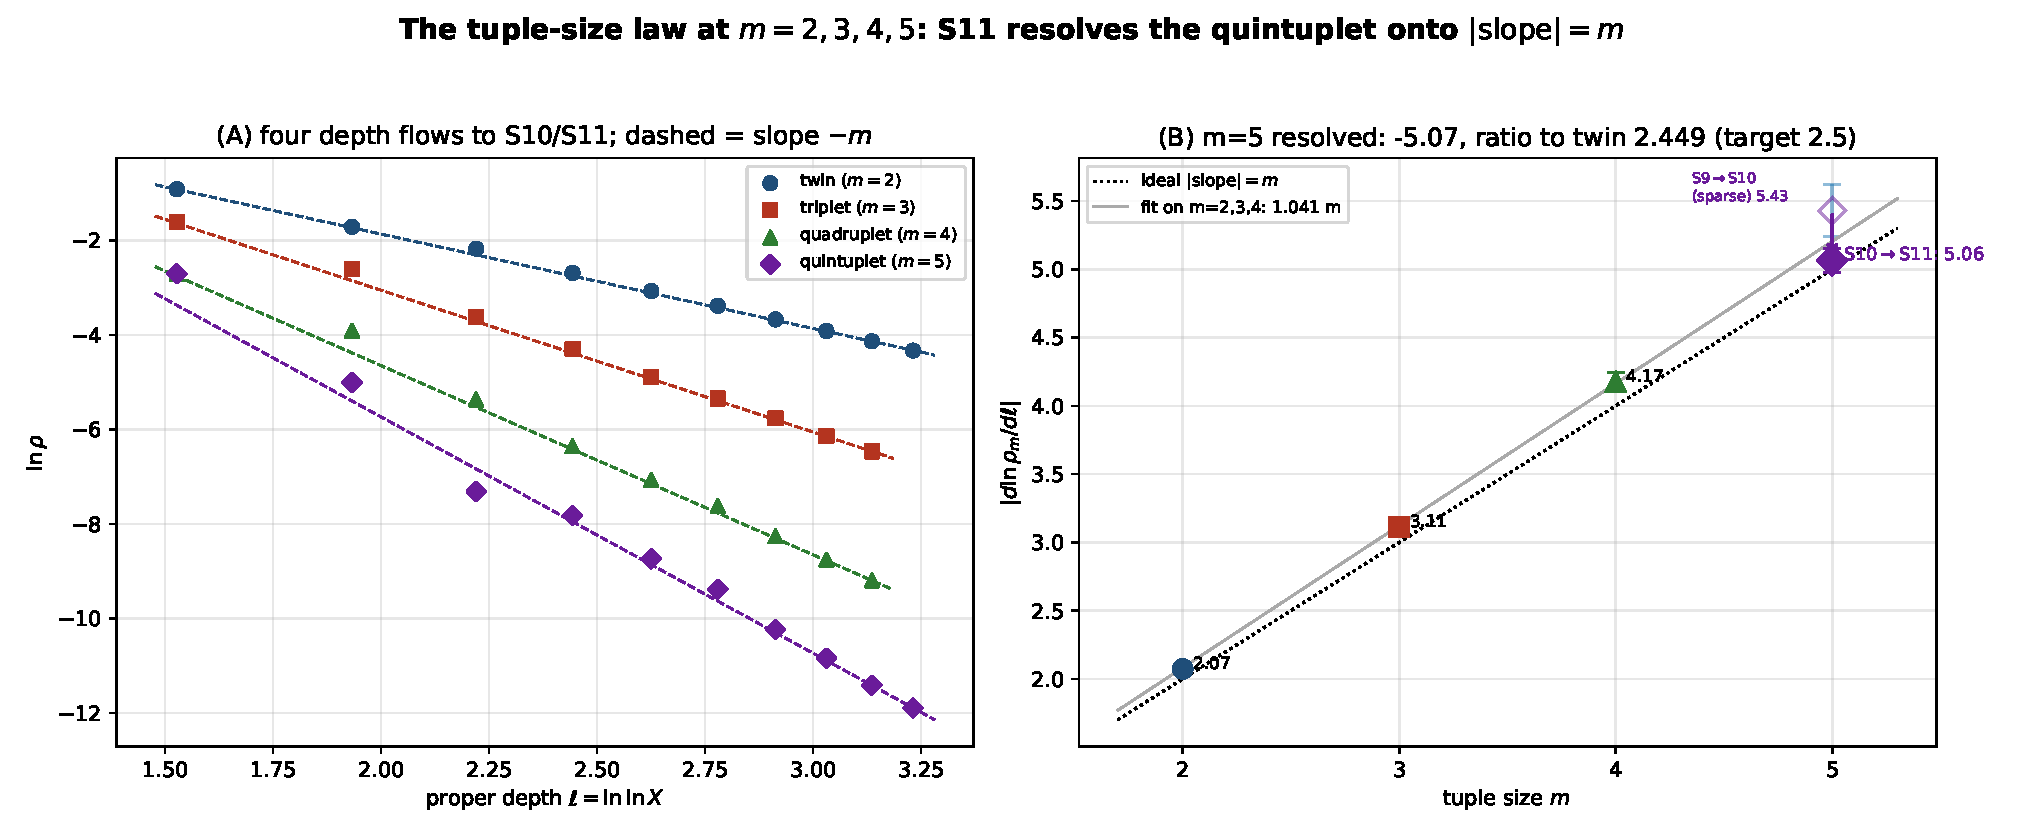
\includegraphics[width=\textwidth]{fig_paper19_tuplelaw_m5.pdf}
\caption{(A) The four depth flows $\ln\rho$ vs $\ell=\ln\ln X$, the quintuplet
extended to $S_{11}$; dashed lines have slope $-m$. (B) The $m=5$ resolution: the
open diamond is the sparsity-limited $S_9\!\to\!S_{10}$ estimate ($5.43$, wide
bar); the arrow shows the descent to $S_{10}\!\to\!S_{11}$ ($5.065$), landing on
$|{\rm slope}|=m$. Ratio to twin $2.449$ against the target $2.5$.}
\label{fig:m5}
\end{figure}

\section{The four-point law}

\begin{theorem}[tuple-size ratio invariant, four points]\label{thm:four}
For prime constellations of sizes $m=2,3,4,5$ on the $6N$ skeleton,
$|d\ln\rho_m/d\ell|=\kappa\,m$ for a single $\kappa$, so the depth-flow slope
ratios are the bare integers $m'/m$. Empirically the ratios to the twin are
\[
  1:1.5011:2.0145:2.4488 \quad\text{against}\quad 1:\tfrac32:2:\tfrac52 ,
\]
the $m=5$ rung confirmed only after descending to $S_{11}$ to escape the
sparse-regime bias. Four points on a line through the origin fix the law: the
topological size of the constellation, and nothing else, sets its stratum decay
rate.
\end{theorem}

The methodological claim of Part~XVIII is also vindicated here. The count-aware
estimator, introduced when the quadruplet first thinned, was stress-tested at
$m=5$ in the sparsest data the series has reached; it did not break, and the
residual bias it could not remove was removed instead by depth. The two
instruments of the sparse regime---weighting and descent---are now both
characterised by where each is needed.

\section{An honest ledger and scope}

As throughout. The flow governs first moments; the $\omega_{>3}$ variance over
twin centres (the Erd\H{o}s--Kac problem of Part~XII~\cite{ChenXII}) is untouched
and remains open. The $(\ln X)^{-m}$ law is the classical Hardy--Littlewood
heuristic~\cite{HL}; $\rho$ is the Part~I scale~\cite{ChenI}. We make no claim
about the infinitude of prime quintuplets or any constellation. A residual
honesty: the quintuplet slope is quoted at a deeper baseline ($S_{10}\!\to\!
S_{11}$) than the others ($S_9\!\to\!S_{10}$); because the twin shifts only from
$-2.072$ to $-2.068$ between these baselines, the comparison is fair to better
than half a percent, and the quoted ratio $2.4488$ uses twin and quintuplet from
the \emph{same} $S_{11}$ pass.

\section{The end of drilling, and the $m=6$ challenge}

This is the last rung we mine. The ladder $m=2,3,4,5$ is ironclad; pursuing $m=6$
is a computational black hole with diminishing theoretical return---the
quintuplet already demanded $S_{11}$ ($\sim2\times10^{11}$ sieved values), and the
sextuplet, an order of magnitude rarer again, would demand $S_{12}$ and beyond.
We therefore state it as a prediction and leave its test to those with the
hardware.

\begin{prediction}[$m=6$, open challenge]\label{pred:m6}
The densest admissible $6$-tuple, the prime sextuplet $(p,p+4,p+6,p+10,p+12,p+16)$,
on the skeleton $(6N+1,6N+5,6N+7,6N+11,6N+13,6N+17)$, must give
$d\ln\rho_6/d\ell\to-6$ and a deep-slope ratio $3{:}1$ against the twin (and
$6{:}5$ against the quintuplet), to the precision at which Theorem~\ref{thm:four}
holds. The test will require shells beyond $S_{11}$ and the count-aware estimator;
a twin ratio outside $3\pm0.07$ would falsify the tuple-size law.
\end{prediction}

\section{Conclusion}

The prime quintuplet supplies the fourth rung, and the manner of its supplying is
the lesson: at the sparse $S_{10}$ baseline the estimate read $-5.43$, overshooting
the law exactly as Part~XVIII warned; descending to $S_{11}$ corrected it to
$-5.065$, ratio $2.4488$, on the bound. The mathematics predicted the bias and
the cure, and the computation obeyed. With four rungs $m=2,3,4,5$ collinear
through the origin and ratios $1:\tfrac32:2:\tfrac52$, the tuple-size law is
established as far as direct enumeration can reasonably reach; the count-aware
estimator and the descent to depth are both validated as the instruments of the
sparse regime. This closes the empirical chapter of the $6N$ programme. The
variance flow remains the open Erd\H{o}s--Kac problem, and $m=6$ stands as the
challenge for larger machines; the law itself, at four points, is no longer a
conjecture in search of confirmation but a measured fact in search of a proof.

\paragraph{Data and code availability.}
The quintuplet counts ($S_2$--$S_{11}$, from scratch), the same-pass twin/quintuplet
recompute, the four-pattern flow analysis with the count-aware estimator, and the
figure are openly available~\cite{repo}; twin/triplet/quadruplet observables are
the Part~I/XV/XVIII tables.

\begin{thebibliography}{9}
\bibitem{HL} G.~H.~Hardy, J.~E.~Littlewood, \emph{Some problems of `Partitio
Numerorum'; III}, Acta Math.\ \textbf{44} (1923), 1--70.
\bibitem{ChenI} R.~Chen, \emph{Prime distribution on the $6N$ skeleton} (Part~I),
Zenodo, doi:10.5281/zenodo.20470367 (2026).
\bibitem{ChenXII} R.~Chen, \emph{The microscopic root $1/(q-2)$ and the mean
shift} (Part~XII), Zenodo, doi:10.5281/zenodo.20528446 (2026).
\bibitem{ChenXVII} R.~Chen, \emph{Arithmetic geodynamics on the $6N$ skeleton}
(Part~XVII), Zenodo, doi:10.5281/zenodo.20541575 (2026).
\bibitem{ChenXVIII} R.~Chen, \emph{The tuple-size law at $m=4$: a prime-quadruplet
confirmation} (Part~XVIII), Zenodo, doi:10.5281/zenodo.20546249 (2026).
\bibitem{repo} R.~Chen, \emph{$6N$ tuple-size law at $m=5$: data and code}
(Part~XIX), \url{https://github.com/Ruqing1963/6N-tuple-law-m5} (2026).
\end{thebibliography}

\end{document}
